%%
%% This is file `tikzposter-template.tex',
%% generated with the docstrip utility.
%%
%% The original source files were:
%%
%% tikzposter.dtx  (with options: `tikzposter-template.tex')
%%
%% This is a generated file.
%%
%% Copyright (C) 2014 by Pascal Richter, Elena Botoeva, Richard Barnard, and Dirk Surmann
%%
%% This file may be distributed and/or modified under the
%% conditions of the LaTeX Project Public License, either
%% version 2.0 of this license or (at your option) any later
%% version. The latest version of this license is in:
%%
%% http://www.latex-project.org/lppl.txt
%%
%% and version 2.0 or later is part of all distributions of
%% LaTeX version 2013/12/01 or later.
%%


\documentclass{tikzposter} %Options for format can be included here

\usepackage{todonotes}

\usepackage[tikz]{bclogo}
\usepackage{lipsum}
\usepackage{amsmath}

\usepackage{booktabs}
\usepackage{longtable}
\usepackage[absolute]{textpos}
\usepackage[it]{subfigure}
\usepackage{graphicx}
\usepackage{cmbright}
%\usepackage[default]{cantarell}
%\usepackage{avant}
%\usepackage[math]{iwona}
\usepackage[math]{kurier}
\usepackage[T1]{fontenc}


%% add your packages here
\usepackage{hyperref}
% for random text
\usepackage{lipsum}
\usepackage[english]{babel}
\usepackage[pangram]{blindtext}

\colorlet{backgroundcolor}{blue!10}

 % Title, Author, Institute
\title{What's Cooking?}
\author{Yuhui Mou}
\institute{Xi'an Shiyou University
}
%\titlegraphic{logos/tulip-logo.eps}

%Choose Layout
\usetheme{Wave}

%\definebackgroundstyle{samplebackgroundstyle}{
%\draw[inner sep=0pt, line width=0pt, color=red, fill=backgroundcolor!30!black]
%(bottomleft) rectangle (topright);
%}
%
%\colorlet{backgroundcolor}{blue!10}

\begin{document}


\colorlet{blocktitlebgcolor}{blue!23}

 % Title block with title, author, logo, etc.
\maketitle

\begin{columns}
 % FIRST column
\column{0.5}% Width set relative to text width

%%%%%%%%%% -------------------------------------------------------------------- %%%%%%%%%%
 %\block{Main Objectives}{
%  	      	\begin{enumerate}
%  	      	\item Formalise research problem by extending \emph{outlying aspects mining}
%  	      	\item Proposed \emph{GOAM} algorithm is to solve research problem
%  	      	\item Utilise pruning strategies to reduce time complexity
%  	      	\end{enumerate}
%%  	      \end{minipage}
%}
%%%%%%%%%% -------------------------------------------------------------------- %%%%%%%%%%


%%%%%%%%%% -------------------------------------------------------------------- %%%%%%%%%%
\block{Introduction}{
    % Many real world applications call for one important function
    % of identifying the set of features
    % on which the interested object is most distinguished from others.
    % Usually,
    % this object is termed as the query object,
    % and the set of features are referred to as the \emph{subspaces} or \emph{aspects}.
    % Accordingly,
    % this research problem is referred to as
    % \emph{outlying aspects mining},
    % which is different from \emph{outlier detection}.
  	
  	% \begin{description}
  	% \item[Outlying Aspects Mining] aims to identify a subspace
    % which makes the query object most outlying,
    % rather than verifying whether it is an outlier or not.
    % The task of \emph{Outlying Aspects Mining}
    % is to explain which aspects make the query object most different.
  	
  	% \item[Outlier Detection] aims to identify all possible outliers in the dataset,
    % without explaining why or how they are different.
    % Hence,
    % the outlying aspects mining is also referred to
    % \emph{outlier interpretation}
    % or \emph{object explanation}.
  	% \end{description}

  	% In this paper,
    % we extend the task of \emph{outlying aspects mining} to the \emph{group} level,
    % formalize the research problem of \emph{group outlying aspects mining},
    % and propose a novel algorithm named GOAM to solve the
    % \emph{group outlying aspects mining} problem.
  There are many countries on the earth, each country has its own characteristic food culture. \\
  China's hot pot,American pizza,Japanese sushi\ldots These are typical food of every country,
  while all these delicious food with different ingredients and different spices.Different food 
  has its own characteristics.Chinese food is rarely used black pepper, 
  while American food love black pepper.So with this project.
  Every foods have their own characteristics of each country.
  In this project,we can distinguish different countries by
  different ingredients.\\
  This is an interesting project.
}
%%%%%%%%%% -------------------------------------------------------------------- %%%%%%%%%%


%%%%%%%%%% -------------------------------------------------------------------- %%%%%%%%%%
\block{Data}{
  This event provides two data sets that can be used: train.json  test.json\\
\begin{itemize}
    \item
    %\emph{Group Outlying Aspects Mining}
    \textbf{train.json}:In the dataset, we include the recipe id, the type of cuisine, and the list of ingredients of each recipe (of variable length). The data is stored in JSON format.
    \item
    \textbf{test.json}:In the test file test.json, the format of a recipe is the same as train.json, only the cuisine type is removed, as it is the target variable you are going to predict.
\end{itemize}

\begin{center}
    \begin{minipage}{0.3\linewidth}
    \centering
    \begin{tikzfigure}
      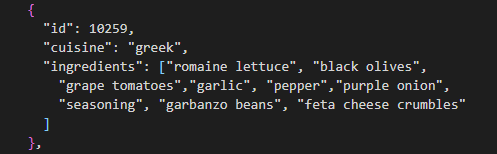
\includegraphics[width=0.9\textwidth]{D://Code//Kaggle-test//Data//train-p.png}
    {\small{train data}}
    \end{tikzfigure}%
    \end{minipage}
    \hfill
    \begin{minipage}{0.3\linewidth}
    \centering
    \begin{tikzfigure}
      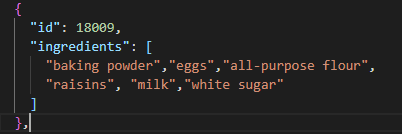
\includegraphics[width=0.9\textwidth]{D://Code//Kaggle-test//Data//test-p.png}
    {\small{test data}}
    \end{tikzfigure}%
    \end{minipage}
    \hfill 
    \begin{minipage}{0.3\linewidth}
      \centering
      \begin{tikzfigure}
        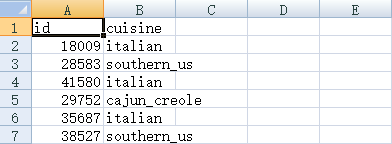
\includegraphics[width=0.9\textwidth]{D://Code//Kaggle-test//Data//out-p.png}
      {\small{Group Outlying Aspects Mining}}
      \end{tikzfigure}%
      \end{minipage}
      
\end{center}
}
%%%%%%%%%% -------------------------------------------------------------------- %%%%%%%%%%


%%%%%%%%%% -------------------------------------------------------------------- %%%%%%%%%%

%\note{Note with default behavior}

%\note[targetoffsetx=12cm, targetoffsety=-1cm, angle=20, rotate=25]
%{Note \\ offset and rotated}

 % First column - second block


%%%%%%%%%% -------------------------------------------------------------------- %%%%%%%%%%
\block{Tool}{\begin{description}
  \item
  BoW\\
  The first Bag of words, also called "word bags", in information retrieval, 
  a Bag of words model assumption for a text, ignore the word order and grammar, 
  syntax, it just as a word set, or the term of a combination of, the emergence of each word in the text are independent, does not depend on whether the other word, or when the author of this article choose a word in an arbitrary position is not affected by the previous sentence and independent choice.
  The first Bag of words, also called "word bags", in information retrieval, a Bag of words model assumption for a text, ignore the word order and grammar, syntax, it just as a word set, or the term of a combination of, the emergence of each word in the text are independent, does not depend on whether the other word, or when the author of this article choose a word in an arbitrary position is not affected by the previous sentence and independent choice.
\end{description}

% \begin{tikzfigure}%[Overall architecture of \emph{GOAM} algorithm]
%     \missingfigure[figcolor=white]{Testing figcolor}
% \end{tikzfigure}
%   where $G_q$ is the query group,
%   $n$ is the number of compare groups,
%   and $h_{k_s}$ is the histogram representation of $G_k$ in the subspace $s$.

\begin{description}
\item 
RandomForestClassifier
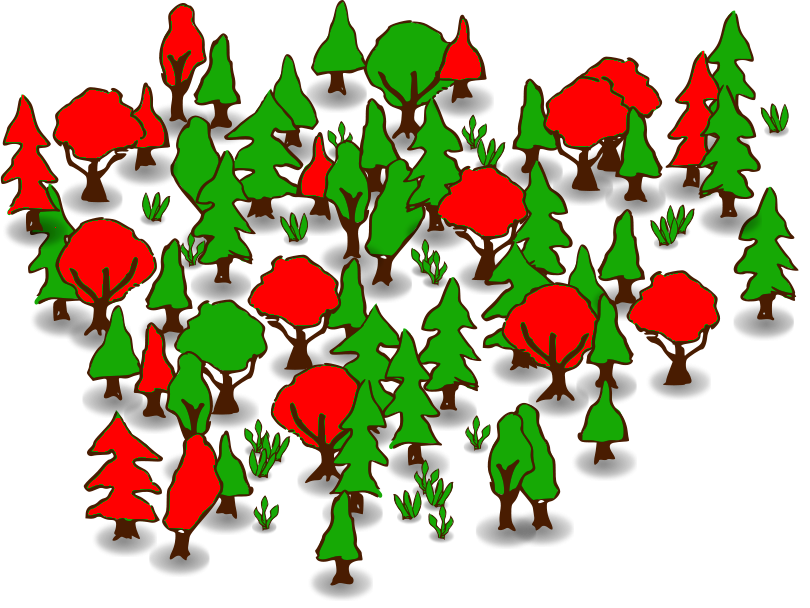
\includegraphics[width=0.2\textwidth]{D://Code//Kaggle-test//Data//suijisenlin.png}\\
There are many classification tree randomly in the forest. We will classify an input samples, we need to input sample input to classify each tree. Make an image of the parable: the meeting in the forest, discuss whether an animal is mouse or squirrel, every tree should be independently published his views on the question, every tree that is voting. This animal is mouse or squirrel, according to vote to determine, won the most votes category is the classification results of the forest. Each tree in the forest are independent, unrelated trees make 99.9\%  of the predicted results to cover all the situation, the forecast results will cancel each other out. A good tree prediction results will be detached from the multitude of "noise", make a good predictions. Several weak classifier classification result vote choice, so as to form a strong classifier, which is the ideas of the random forest bagging
  
\end{description}
  
%   	We propose the \emph{GOAM} algorithm to solve the research problem of
%     \emph{Group Outlying Aspects Mining}.
%   	The \emph{GOAM} algorithm includes three major steps.
% %    1) Group Feature Extraction,
% %    2) Outlying Degree Scoring, and
% %    3) Outlying Aspects Identification.
  	
% \begin{tikzfigure}%[Overall architecture of \emph{GOAM} algorithm]
% %  \includegraphics[width=0.8\linewidth]{figures//framework.pdf}
%     \missingfigure[figcolor=white]{Testing figcolor}
% \end{tikzfigure}
		
% \begin{description}
%   	\item[Group Feature Extraction]
%   	Let $f_1$, $f_2$, $f_3$ represent three features of $G_q$.
%     We count the frequency of each value for one feature.
%     Then use the histogram to represent each feature.
%     Similarly,
%     we can extract other features for each group.

% %    \item
% %    The histogram of $G_q$ on three features are as follows.
% \end{description}

% \begin{center}
%     \begin{minipage}{0.3\linewidth}
%     \centering
%     \begin{tikzfigure}
%     \missingfigure[figcolor=white]{Testing figcolor}
%     {\small{Histogram of $G_q$ on $f_1$}}
%     \end{tikzfigure}%
%     \end{minipage}
%     \hfill
%     \begin{minipage}{0.3\linewidth}
%     \centering
%     \begin{tikzfigure}
%     \missingfigure[figcolor=white]{Testing figcolor}
%     {\small{Histogram of $G_q$ on $f_2$}}
%     \end{tikzfigure}%
%     \end{minipage}
%     \hfill
%     \begin{minipage}{0.3\linewidth}
%     \centering
%     \begin{tikzfigure}
%     \missingfigure[figcolor=white]{Testing figcolor}
%     {\small{Histogram of $G_q$ on $f_3$}}
%     \end{tikzfigure}%
%     \end{minipage}
% \end{center}
% \begin{description}
% \item[Outlying Degree Scoring]
%     In this step,
%     we first calculate the \emph{earth mover distance} (EMD) of one feature among different groups.
%     The earth mover distance reflects the minimum mean distance
%     between groups on one feature.
%     So,
%     we utilize the EMD to measure the difference between groups of each feature.
% \end{description}

}
%%%%%%%%%% -------------------------------------------------------------------- %%%%%%%%%%


% SECOND column
\column{0.5}
 %Second column with first block's top edge aligned with with previous column's top.

%%%%%%%%%% -------------------------------------------------------------------- %%%%%%%%%%
\block{Data Processing}{
  \begin{itemize}
    \item
    Read Data \\
  \begin{itemize}
  \item
  Read train.json
  \item
  Read test.json
  \end{itemize}
  \item
  Processing Model:Bag-of-words model (BoW model)\\
  \begin{itemize}
    \item 
    BoW early in Natural Language Processing and Information Retrieval 
    This model ignored the grammar and word order elements such as text, 
    just as it is a collection of several words, the emergence of each
     word in the document are independent of each otherBoW to use an 
     unordered list of words to express a text or a document.
  \end{itemize}
  \begin{itemize}
    \item 
    CountVectorizer is a characteristic class of common numerical calculation,
    Is a text feature extraction method.For each training text, it only considers 
    each of these words in the frequency of the training in the text.
    CountVectorizer Converts text of the words in the word frequency matrix.
    
  \end{itemize}
  \item 
RandomForestClassifier\\
  \begin{itemize}
  \item
  The first step is using feature and target training classifier.
  \item
  The second step is to input data to classifier which has trained before.
  \item 
  Export data and Store them in a document.
  \end{itemize}

    %\emph{Group Outlying Aspects Mining}
  
\end{itemize}
}
%%%%%%%%% -------------------------------------------------------------------- %%%%%%%%%%
% Second column - first block


%%%%%%%%%% -------------------------------------------------------------------- %%%%%%%%%%
% \block[titleleft]{Experiment}
% {
% \begin{description}
%   	\item[Synthetic Dataset] contains $10$ groups and $8$ features.
%     Each group consists of $10$ members,
%     and each member has $8$ features.
% \end{description}
% \vspace{.5cm}
% \begin{tabular}{ c | c | c | c }
%     \toprule
%     Method     &  Truth Outlying Aspects    & Identified Aspects & Accuracy      \\
%     \midrule
%     GOAM       &  $\{F_1\}$, $\{F_2F_4\}$   &  $\{F_1\}$, $\{F_2F_4\}$    & 100\%    \\

%      Arithmetic Mean based OAM &  $\{F_1\}$, $\{F_2F_4\}$   &  $\{F_4\}$, $\{F_2\}$    &  0\% \\

%      Median based OAM &  $\{F_1\}$, $\{F_2F_4\}$   &  $\{F_2\}$, $\{F_4\}$    &           0\% \\
%      \bottomrule
% \end{tabular}
% \vspace{.2cm}
% \begin{description}
%     \item
%     It can be observed that the GOAM method can identify the trivial outlying features
%     and non-trivial outlying subspaces correctly and is obvious from the table
%     that the accuracy of GOAM is the best, which is ($100\%$).
% \end{description}

% \begin{description}
% \item[NBA Dataset] was collected from Yahoo Sports
% website (\url{http://sports.yahoo.com.cn/nba}).
% The data include all teams from the six divisions,
% and each player in the team has $12$ features.
% \end{description}
% \vspace{.5cm}
% \begin{tabular}{ c | c | c }
%     \toprule
%     Teams                   & Trivial Outlying Aspects  & NonTrivial Outlying Aspects    \\
%     \toprule
%     Cleveland Cavaliers     & \{3FA\}                   & \{FGA, FT\%\}, \{FGA, FG\%\} \\
%     Orlando Magic           & \{Stl\}                   & None                         \\
%     Milwaukee Bucks         & \{To\}, \{FTA\}           & \{FGA, FTA\}, \{3FA, FTA\}     \\
% %    Golden State Warriors   & \{FG\%\}                  & \{FT\%, Blk\}, \{FGA, 3PT\%, FTA\}\\
% %    Utah Jazz               & \{Blk\}                   & \{3FA, 3PT\%\}                    \\
%     New Orleans Pelicans    & \{FT\%\}, \{FTA\}         & \{FTA, Stl\}, \{FTA, To\}          \\
%     \bottomrule
% \end{tabular}
           
% \begin{minipage}{0.5\linewidth}
%     \centering
%     \begin{tikzfigure}
%     \missingfigure[figcolor=white]{Testing figcolor}

%     {\small{New Orleans Pelicans on FT\%}}
%     \end{tikzfigure}%
% \end{minipage}
% \hfill
% \begin{minipage}{0.5\linewidth}
%     \centering
%     \begin{tikzfigure}
%     \missingfigure[figcolor=white]{Testing figcolor}

%     {\small{New Orleans Pelicans on FTA}}
%     \end{tikzfigure}%
% \end{minipage}
% \vspace{.2cm}
% \begin{description}
% \item
% \texttt{New Orleans Pelicans} has more players with
% lower \{free throw percentage\}, \{free throws attempted\}.
% \end{description}
% }
%%%%%%%%%% -------------------------------------------------------------------- %%%%%%%%%%


% Second column - second block
%%%%%%%%%% -------------------------------------------------------------------- %%%%%%%%%%
\block[titlewidthscale=1, bodywidthscale=1]
{Conclusion}
{
\begin{description}
  \item 
  Every country has its specialties,each cuisine has it's own ingredients.During this competition,I learned how to
identify the country by different ingredients.At the same time, I also learned how to deal with plain text data set-
BoW model,besides,CountVectorizer is also a great way to extracting text feature.In the end,using feature we extarcted to
classify in RandomForestClassifier.
\end{description}
}
%%%%%%%%%% -------------------------------------------------------------------- %%%%%%%%%%


% Bottomblock
%%%%%%%%%% -------------------------------------------------------------------- %%%%%%%%%%
\colorlet{notebgcolor}{blue!20}
\colorlet{notefrcolor}{blue!20}
\note[targetoffsetx=8cm, targetoffsety=-4cm, angle=30, rotate=15,
radius=2cm, width=.26\textwidth]{
Acknowledgement
\begin{itemize}
  \item 
  We want to thank Yummly for providing this unique dataset. Kaggle is hosting this playground competition for fun and practice.
  The authors would like to thank \ldots
 \end{itemize}
}

%\note[targetoffsetx=8cm, targetoffsety=-10cm,rotate=0,angle=180,radius=8cm,width=.46\textwidth,innersep=.1cm]{
%Acknowledgement
%}

%\block[titlewidthscale=0.9, bodywidthscale=0.9]
%{Acknowledgement}{
%}
%%%%%%%%%% -------------------------------------------------------------------- %%%%%%%%%%

\end{columns}


%%%%%%%%%% -------------------------------------------------------------------- %%%%%%%%%%
%[titleleft, titleoffsetx=2em, titleoffsety=1em, bodyoffsetx=2em,%
%roundedcorners=10, linewidth=0mm, titlewidthscale=0.7,%
%bodywidthscale=0.9, titlecenter]

%\colorlet{noteframecolor}{blue!20}
% \colorlet{notebgcolor}{blue!20}
% \colorlet{notefrcolor}{blue!20}
% \note[targetoffsetx=-13cm, targetoffsety=-12cm,rotate=0,angle=180,radius=8cm,width=.96\textwidth,innersep=.4cm]
% {
% % \begin{minipage}{0.3\linewidth}
% % \centering
% % \includegraphics[width=24cm]{logos/tulip-wordmark.eps}
% % \end{minipage}
% \begin{minipage}{0.7\linewidth}
% { \centering
%  The $11^{th}$ International Conference on Knowledge Science,
%   Engineering and Management (KSEM 2018),
%   17-19/08/2018, Changchun, China
% }
% \end{minipage}
% }
%%%%%%%%%% -------------------------------------------------------------------- %%%%%%%%%%


\end{document}

%\endinput
%%
%% End of file `tikzposter-template.tex'.
